\chapter{Analyse de l'architecture modulaire, champs d'application}

\graphicspath{{03-Algorithme/}}

Avant de pouvoir étudier une architecture de cartes, il est nécessaire de se pencher sur les outils de visualisation de ces cartes, ainsi que sur les indicateurs qu'on peut étudier pour qualifier les comportement. 
Il faut noter qu'une carte de Kohonen, malgré son fonctionnement apparemment simple, se montre compliquée lorsqu'il s'agit de l'étudier mathématiquement. On peut donc seulement citer les études proposées par (Cottrell, 2003) a propos de la convergence d'une carte 1D. Les auteurs se posent les questions suivantes: 
\begin{itemize}
\item Est ce que la carte converge ? 
\item Comment savoir si une représentation apportée par la carte est pertinente ?  
\end{itemize}

Dans le cas d'une carte 1D, on cherche ces réponses mathématiquement mais les représentation usuelle des cartes permet une intuition du résulat : on a de fortes chances d'avoir juste en supposant que la carte converge. Quant à la représentation, on peut proposer des interprétation visuelles : si la carte couvre toutes les données, si elle est "bien dépliée" à l'oeil, l'apprentissage semble pertinent.

Dans le cas de l'architecture CxSOM, on se trouve dans une situation épineuse : même la visualisation des poids ne permet pas de conclure et savoir si on a bien représenté les entrées. 


\section{Cas d'utilisation : les entrées multimodales}

\subsection{Définition et inspiration biologique}



\subsection{Formalisme}



\subsection{Perspectives}

Le formalisme présenté, avec des entrées multimodale comme fonction de variable cachées n'est pas forcément général.  

\section{Représentation des entrées}



\section{Information apprise par une carte}

Une idée est de déterminer si une carte a gagné de l'information sur le modèle générant les entrées. Dans le cas simple, ce modèle peut être entièrement reprénté par $U$; chaque carte peut être représentée par son BMU, considéré comme la seule sortie de la carte. 
En tracant $U$ en fonction de $\Pi$, le BMU d'une carte, on observe directement si une carte a été capable de lever l'ambiguité sur le modèle en distinguant les entrées selon leur variable cachée $U$. Cette ambiguité est levée si $U$ est une fonction de $\Pi$. Cette fonction est observée dans le cas des cartes jointes.

Cette propriété, dans le cas 1D, peut être calculée par l'information mutuelle entre $U$ et $\Pi$. Plus précisément, par $\frac{I(U,\Pi)}{H(U)}$, avec $H(U)$ l'entropie de $U$. 
En effet, dans le meilleurs des cas, $U$ est une fonction parfaite de $\Pi$ et donc $H(U|\Pi ) = 0$ : en connaissant $\Pi$, on connait totalement $U$. Alors, $I(U,\Pi) = H(U) - H(U| \Pi) = H(U)$. 
Notre indicateur vaut alors 1 lorsque $U$ est une fonction parfaite de $\Pi$.
De plus $\Pi$ est forcément une fonction de $U$ car l'algorithme est déterministe: à une entrée correspond une sortie, toujours la même, donc $(I(U, \Pi) = H(\Pi)$. Notre indicateur estimant l'information portée par le BMU d'une carte sur la variable cachée du modèle U est donc $$\frac{H(\Pi)}{H(U)}$$.

Cet indicateur doit être estimé en discrétisant les variables, donnant une entropie nécessairement positive et strictement supérieure à 0.
L'évolution de l'indicateur au cours de l'apprentissage est donnée en figure \ref{fig:im}. Cet indicateur est calculé en moyenne pour 100 réalisations de l'apprentissage, avec des poids initiaux différents. 

\begin{figure}
\centering
\includegraphics[width = \textwidth]{XU_YU.pdf}
\caption{Pour l'échantillon de test, valeur de $U$ en fonction des valeurs du BMU $\Pi$ dans chacune des cartes. On voit que $U$ est une fonction du BMU dans chaque carte, contrairement au cas ou les cartes apprendraient indépendamment sur les mêmes entrées, voir figure \ref{fig:piu_indep}.}
\label{fig:piu}
\end{figure}

\begin{figure}
\centering
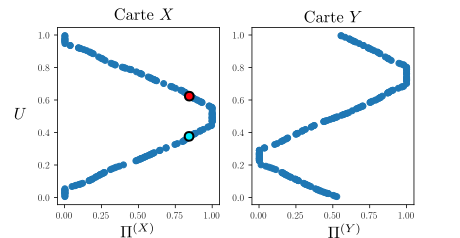
\includegraphics[width = \textwidth]{xu_yu_unco.pdf}
\caption{Pour l'échantillon de test, entrée sur un cercle, valeur de $U$ en fonction des valeurs du BMU $\Pi$ dans chacune des cartes, lorsque les cartes $M_x$ et $M_y$ ne sont pas connectée. Chacune des cartes n'a aucune information de plus que celle portée par son entrée sur l'état global du système $U$, et $\Pi$ n'est donc pas une fonction de $U$ dans chaque carte. }
\label{fig:piu_indep}
\end{figure}

\begin{figure}
\centering
\includegraphics[width=\textwidth]{mutual_info_evol.pdf}
\caption{Evolution de l'indicateur relatif à l'information mutuelle entre $\Pi$ et $U$ dans chaque carte au cours de l'apprentissage. Cet indicateur est comparé à celui calculé dans le cas ou les cartes apprennent séparément.}
\label{fig:im} 
\end{figure}

\textcolor{red}{
\paragraph{Choses à faire}
\begin{itemize}
\item Cette valeur est uniquement calculée pour un modèle connu, et en 1 dimension forcément. Peut on avoir des équivalents en plus de dimension ? 
\item Il existe des quantités mesurant l'information portée par un symbole sur une variable, une sorte d'info mutuelle locale. On sait que $I(U,\Pi) = H(\Pi)$, et on veut que $I(U,\Pi) = H(U)$, mais comment est elle répartie entre les BMUs ? Est-ce pertinent de se pencher sur ces quantités ? 
\end{itemize}
}


\section{Représenter une carte au sein d'une architecture}

Représentation des poids, des entrées, des BMU - analyse




\section{Choix des paramètres}

\subsection{Influence des rayons de voisinage}

\subsection{Influence des autres paramètres}

\subsection{Compatibilité en 2D}

\section{Analyse de la relaxation}

L'apprentissage conjoint des cartes repose sur la relaxation au sein d'une itération. On cherche donc à vérifier si la relaxation converge vers une valeur quelle que soit l'entrée, et si elle est pertinente en large dimension avec de nombreuses cartes.

\subsection{Analyse expérimentale}

\subsection{Champs de BMU}

\subsection{Limitations et possibilités en grande dimension}

\section{Implémentation}

L'implémentation des expériences a été réalisée via l'environnement CxSOM \cite{cxsom}.

\section{Perspectives d'évolutions}


Avant de présenter les performances d'un algorithme, il s'agit de définir plus précisément ce qu'on attend de ce système et comment le représenter. L'architecture CxSOM se présente comme une construction qui répond à un questionnement structurel des réseaux de neurones. Mais au juste, qu'attend t-on de ce réseau de neurones ? De la prédiction, de l'organisation ? Les cartes de Kohonen sont habituellement utilisées dans un objectif de clustering, ou associées à d'autres algorithmes de prédiction utilisant leurs propriétés structurelles. En étude préliminaire pour CxSOM, il s'agit de comprendre le comportement de l'architecture de cartes.

